The controller layer holds the raspberry pi and drone database subsystem.  The raspberry pi controls much of the system's features, as well as acting as an interface between the different layers.  The drone database holds all the processed data and sends the information to users.

\begin{figure}[h!]
	\centering
 	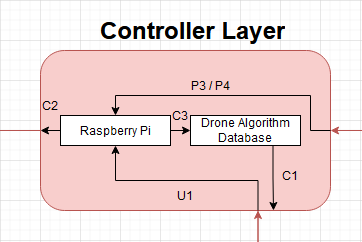
\includegraphics[width=0.50\textwidth]{images/controller.png}
 \caption{Controller subsystems diagram}
\end{figure}

\subsection{Raspberry Pi}
In this system, the Raspberry Pi acts as the central hub that controls the traffic of data flow from one subsystem to another. It also activates functions of specific subsystems based on feedback from another subsystem.

\subsubsection{Assumptions}
The Raspberry Pi is assumed to be powered on throughout the active run time of the system. In addition to that, the Pi needs to have a persistent forms of connections with the other subsystems.

\subsubsection{Responsibilities}
Here is an overview of the data flow pathways that Pi is involved in:
\begin{itemize}
  \item After receiving a positive signal of drone detection from ODAS (which is in the Processing Subsystem), the Pi activates the secondary detector in the Detection Subsystem. 
  \item After receiving confirmation of drone detection from Secondary Processor, it relays relevant drone data to the Drone Algorithm Database.
  \item The Pi also has a bi-directional connection with I/O Subsystems, particularly with the Application subsystem. It is the point of contact in terms of setting updates and user-logins for the user of the system.
\end{itemize}

\subsubsection{Subsystem Interfaces}
Each of the inputs and outputs for the subsystem are defined here. 

\begin {table}[H]
\caption {Raspberry Pi Interfaces} 
\begin{center}
    \begin{tabular}{ | p{2cm} | p{5cm} | p{3cm} | p{4cm} |}
    \hline
    ID & Description & Inputs & Outputs \\ \hline
    \#P4 and C2 & Activation of secondary detector & \pbox{3cm}{Signal from ODAS confirming drone presence (P4)} & \pbox{4cm}{Activation of secondary sensor in Detection subsystems (C2)}  \\ \hline
    \#P3 and C3 & Relaying drone information to database & \pbox{3cm}{Signal from secondary processor (P2)} & \pbox{4cm}{Drone data relayed to Drone Algorithm Database (C3)}  \\ \hline
    \#U1 & User interactions relayed by Raspberry Pi & \pbox{3cm}{User inputs from Application} & \pbox{4cm}{Feedback after processing user inputs back to Application}  \\ \hline
    \end{tabular}
\end{center}
\end{table}

\subsection{Drone Algorithm Database}
The drone algorithm database stores and manages captured drone data, so that it can be accessed by the application and displayed in a readable format. Logically, it makes sense to have a closer proximity to the controller layer, since most its interactions with other layers and subsystems would be overseen by the Raspberry Pi (the controller of the system).
\subsubsection{Assumptions}
The database is assumed to have a persistent connection in the system's network and the internet. It should be free of any major security issues when data is loaded or accessed by any other subsystem.
\subsubsection{Responsibilities}
Here is an overview of the database's functionality, other than managing the stored data:
\begin{itemize}
  \item Whenever a new update in drone detection is confirmed by the Pi, it relays relevant information on the detected drone to the database. This is the primary interface through which the database receives updates.
  \item The other interface link is between the database and the application subsystem in the I/O layer. The application accesses the database through this link to retrieve drone data that it eventually displays to its user.
\end{itemize}
\subsubsection{Subsystem Interfaces}
\begin {table}[H]
\caption {Drone Algorithm Database interfaces} 
\begin{center}
    \begin{tabular}{ | p{1cm} | p{6cm} | p{3cm} | p{4cm} |}
    \hline
    ID & Description & Inputs & Outputs \\ \hline
    \#C1 & Access link between application and database & \pbox{3cm}{Access request by application \\} & \pbox{4cm}{Fulfillment of access request}  \\ \hline
    \#C3 & Reception of new drone data & \pbox{3cm}{Information relayed by Pi} & \pbox{4cm}{Updated database}  \\ \hline
    \end{tabular}
\end{center}
\end{table}

